% Options for packages loaded elsewhere
\PassOptionsToPackage{unicode}{hyperref}
\PassOptionsToPackage{hyphens}{url}
\documentclass[11pt]{article}
\usepackage{amsmath,amssymb}
\usepackage{iftex}
\ifPDFTeX
  \usepackage[T1]{fontenc}
  \usepackage[utf8]{inputenc}
  \usepackage{textcomp} % provide euro and other symbols
\else % if luatex or xetex
  \usepackage{unicode-math} % this also loads fontspec
  \defaultfontfeatures{Scale=MatchLowercase}
  \defaultfontfeatures[\rmfamily]{Ligatures=TeX,Scale=1}
\fi
\usepackage{lmodern}

% Custom modern typography and page layout
\usepackage[letterpaper, margin=1in]{geometry}
\usepackage{xcolor}
\usepackage{colortbl}
\usepackage{fancyhdr}
\usepackage{titlesec}
\usepackage{enumitem}

% Color palette definition
\definecolor{DeepNavy}{HTML}{1A365D}
\definecolor{SlateBlue}{HTML}{2B6CB0}
\definecolor{Charcoal}{HTML}{2D3748}
\definecolor{LightGray}{HTML}{F7FAFC}
\definecolor{TableLine}{HTML}{CBD5E0}
\definecolor{AccentGold}{HTML}{D69E2E}

% Modern section styling
\titleformat{\section}
  {\color{DeepNavy}\normalfont\Large\bfseries}
  {\thesection}{1em}{}[{\color{DeepNavy}\titlerule[0.8pt]}]
\titleformat{\subsection}
  {\color{SlateBlue}\normalfont\large\bfseries}
  {\thesubsection}{1em}{}
\titleformat{\subsubsection}
  {\color{Charcoal}\normalfont\normalsize\bfseries}
  {\thesubsubsection}{1em}{}

% Headers and Footers configuration
\pagestyle{fancy}
\fancyhf{}
\fancyhead[L]{\color{Charcoal}\small\itshape Plan de Implementación de Habilitadores --- APO02}
\fancyhead[R]{\color{Charcoal}\small Eco Logistic S.A.C.}
\fancyfoot[C]{\color{Charcoal}\thepage}
\renewcommand{\headrulewidth}{0.4pt}
\renewcommand{\footrulewidth}{0pt}

% Keep other pandoc package configurations for compatibility
\IfFileExists{upquote.sty}{\usepackage{upquote}}{}
\IfFileExists{microtype.sty}{% use microtype if available
  \usepackage[]{microtype}
  \UseMicrotypeSet[protrusion]{basicmath} % disable protrusion for tt fonts
}{}

\usepackage{longtable,booktabs,array}
\newcounter{none} % for unnumbered tables
\usepackage{multirow}
\usepackage{calc} % for calculating minipage widths
% Correct order of tables after \paragraph or \subparagraph
\usepackage{etoolbox}
\makeatletter
\patchcmd\longtable{\par}{\if@noskipsec\mbox{}\fi\par}{}{}
\makeatother
% Allow footnotes in longtable head/foot
\IfFileExists{footnotehyper.sty}{\usepackage{footnotehyper}}{\usepackage{footnote}}
\makesavenoteenv{longtable}
\usepackage{graphicx}
\makeatletter
\newsavebox\pandoc@box
\newcommand*\pandocbounded[1]{% scales image to fit in text height/width
  \sbox\pandoc@box{#1}%
  \Gscale@div\@tempa{\textheight}{\dimexpr\ht\pandoc@box+\dp\pandoc@box\relax}%
  \Gscale@div\@tempb{\linewidth}{\wd\pandoc@box}%
  \ifdim\@tempb\p@<\@tempa\p@\let\@tempa\@tempb\fi% select the smaller of both
  \ifdim\@tempa\p@<\p@\scalebox{\@tempa}{\usebox\pandoc@box}%
  \else\usebox{\pandoc@box}%
  \fi%
}
% Set default figure placement to htbp
\def\fps@figure{htbp}
\makeatother
\setlength{\emergencystretch}{3em} % prevent overfull lines
\providecommand{\tightlist}{%
  \setlength{\itemsep}{0pt}\setlength{\parskip}{0pt}}
\usepackage{bookmark}
\IfFileExists{xurl.sty}{\usepackage{xurl}}{} % add URL line breaks if available
\urlstyle{same}
\hypersetup{
  hidelinks,
  pdfcreator={LaTeX via pandoc}}

\author{}
\date{}

\begin{document}

% Portada Corporativa Premium
\begin{titlepage}
  \thispagestyle{empty}
  \centering
  
  \vspace*{0.5cm}
  {\scshape\Large\bfseries UNIVERSIDAD PERUANA UNIÓN \par}
  {\scshape\large Facultad de Ingeniería y Arquitectura \par}
  {\scshape\normalsize Escuela Profesional de Ingeniería de Sistemas \par}
  
  \vspace{1.0cm}
  
\includegraphics[width=2.2in,height=1.85in,keepaspectratio]{media/image1.png}
  \vspace{1.0cm}
  
  {\color{DeepNavy}\hrule height 2pt}
  \vspace{0.4cm}
  {\Huge\bfseries PLAN DE IMPLEMENTACIÓN DE HABILITADORES \par}
  \vspace{0.2cm}
  {\Large\bfseries Proceso COBIT: APO02 --- Gestionar la Estrategia \par}
  \vspace{0.4cm}
  {\color{AccentGold}\hrule height 1pt}
  \vspace{0.4cm}
  {\Large\bfseries ``Optimizar Procesos Logísticos con WMS/ERP en la Nube'' \par}
  \vspace{0.2cm}
  {\large\bfseries CO LOGISTIC S.A.C. \par}
  \vspace{0.4cm}
  {\color{DeepNavy}\hrule height 2pt}
  
  \vspace{1.2cm}
  
  \begin{minipage}[t]{0.55\textwidth}
    \begin{flushleft} \large
      \textbf{Integrantes:}\\
      \smallskip
      \small
      Jhack Ernesto Quispe Mamani\\
      Abel Is-Boset Guevara Huasco\\
      Javier Kevin Tello Rivas\\
      Richard Joseft Yanqui Inocente\\
      Alvaro Kenji Cuti Magaño\\
      David Guerra Ordoñez\\
      Joshua Alfonzo Javier\\
      Sebastían Chinchay Collachagua
    \end{flushleft}
  \end{minipage}
  \hfill
  \begin{minipage}[t]{0.38\textwidth}
    \begin{flushright} \large
      \textbf{Docente:}\\
      \smallskip
      \small Lennin Henry Centurion Julca \\
      \vspace{0.4cm}
      \textbf{Curso:}\\
      \smallskip
      \small Gobierno de TI \\
      \vspace{0.4cm}
      \textbf{Ciclo:} \small 9no \\
      \vspace{0.4cm}
      \textbf{Versión:} \small 1.0
    \end{flushright}
  \end{minipage}
  
  \vfill
  
  {\large Lima --- Perú \par}
  {\large 2026 \par}
\end{titlepage}

\newpage
\pagenumbering{roman}
\thispagestyle{plain}
\tableofcontents
\newpage
\pagenumbering{arabic}

\section*{Resumen Ejecutivo}
\addcontentsline{toc}{section}{Resumen Ejecutivo}

CO LOGISTIC S.A.C. presenta la necesidad de fortalecer su gestión estratégica de TI debido a problemas relacionados con la trazabilidad de inventarios, ubicabilidad de productos, dependencia de registros manuales o plataformas informales, y falta de estandarización documental en sus procesos logísticos internos.

Frente a esta situación, se propone implementar el proceso APO02 --- Gestionar la Estrategia, basado en COBIT, con el propósito de ordenar, formalizar y controlar la estrategia de TI denominada ``Optimizar procesos logísticos con WMS/ERP en la nube''. Esta estrategia se encuentra alineada con dos estrategias principales del negocio: implementar un sistema de trazabilidad de inventarios que elimine los problemas de ubicabilidad y estandarizar los procesos logísticos internos para reducir la dependencia de plataformas externas informales y garantizar la continuidad operativa.

El presente documento establece una hoja de trabajo para implementar APO02 en CO LOGISTIC S.A.C., considerando seis fases: preparación e inicio, evaluación y diseño, construcción y pruebas, implementación y transición, operación y medición, y optimización y mejora continua. Asimismo, se incluyen elementos de gobierno de TI como alineamiento estratégico, matriz RACI, indicadores, riesgos estratégicos, roadmap tecnológico, evidencias documentales y mecanismos de seguimiento.

La propuesta busca que la empresa pase de una gestión logística parcialmente manual y poco integrada hacia un modelo más formal, trazable, medible y sostenible, apoyado por una solución WMS/ERP en la nube, tableros de indicadores y procesos documentados.

CO LOGISTIC S.A.C. es una empresa vinculada a actividades logísticas, donde la trazabilidad, el control de inventarios, la correcta ubicación de productos, la gestión de documentos y la continuidad operativa son elementos fundamentales para asegurar un servicio eficiente y confiable.

Actualmente, la empresa cuenta con iniciativas orientadas a mejorar sus operaciones; sin embargo, todavía presenta oportunidades de mejora en la formalización de sus procesos, en el uso de herramientas tecnológicas integradas y en el seguimiento estratégico de sus iniciativas de TI. La existencia de registros manuales, archivos en Excel, documentos estratégicos en proceso de formalización y antecedentes de iniciativas tecnológicas no consolidadas evidencia la necesidad de fortalecer la gestión estratégica de TI.

En este contexto, la implementación del proceso APO02 permitirá que CO LOGISTIC gestione de manera formal su estrategia tecnológica, priorizando iniciativas que aporten valor directo al negocio. La estrategia seleccionada es la optimización de procesos logísticos mediante un WMS/ERP en la nube, orientado a mejorar la trazabilidad, la ubicabilidad, la estandarización de procesos y la continuidad operativa.

\vspace{0.4cm}
\textbf{Estrategias de negocio y estrategia de TI:}

\begin{center}
  \pandocbounded{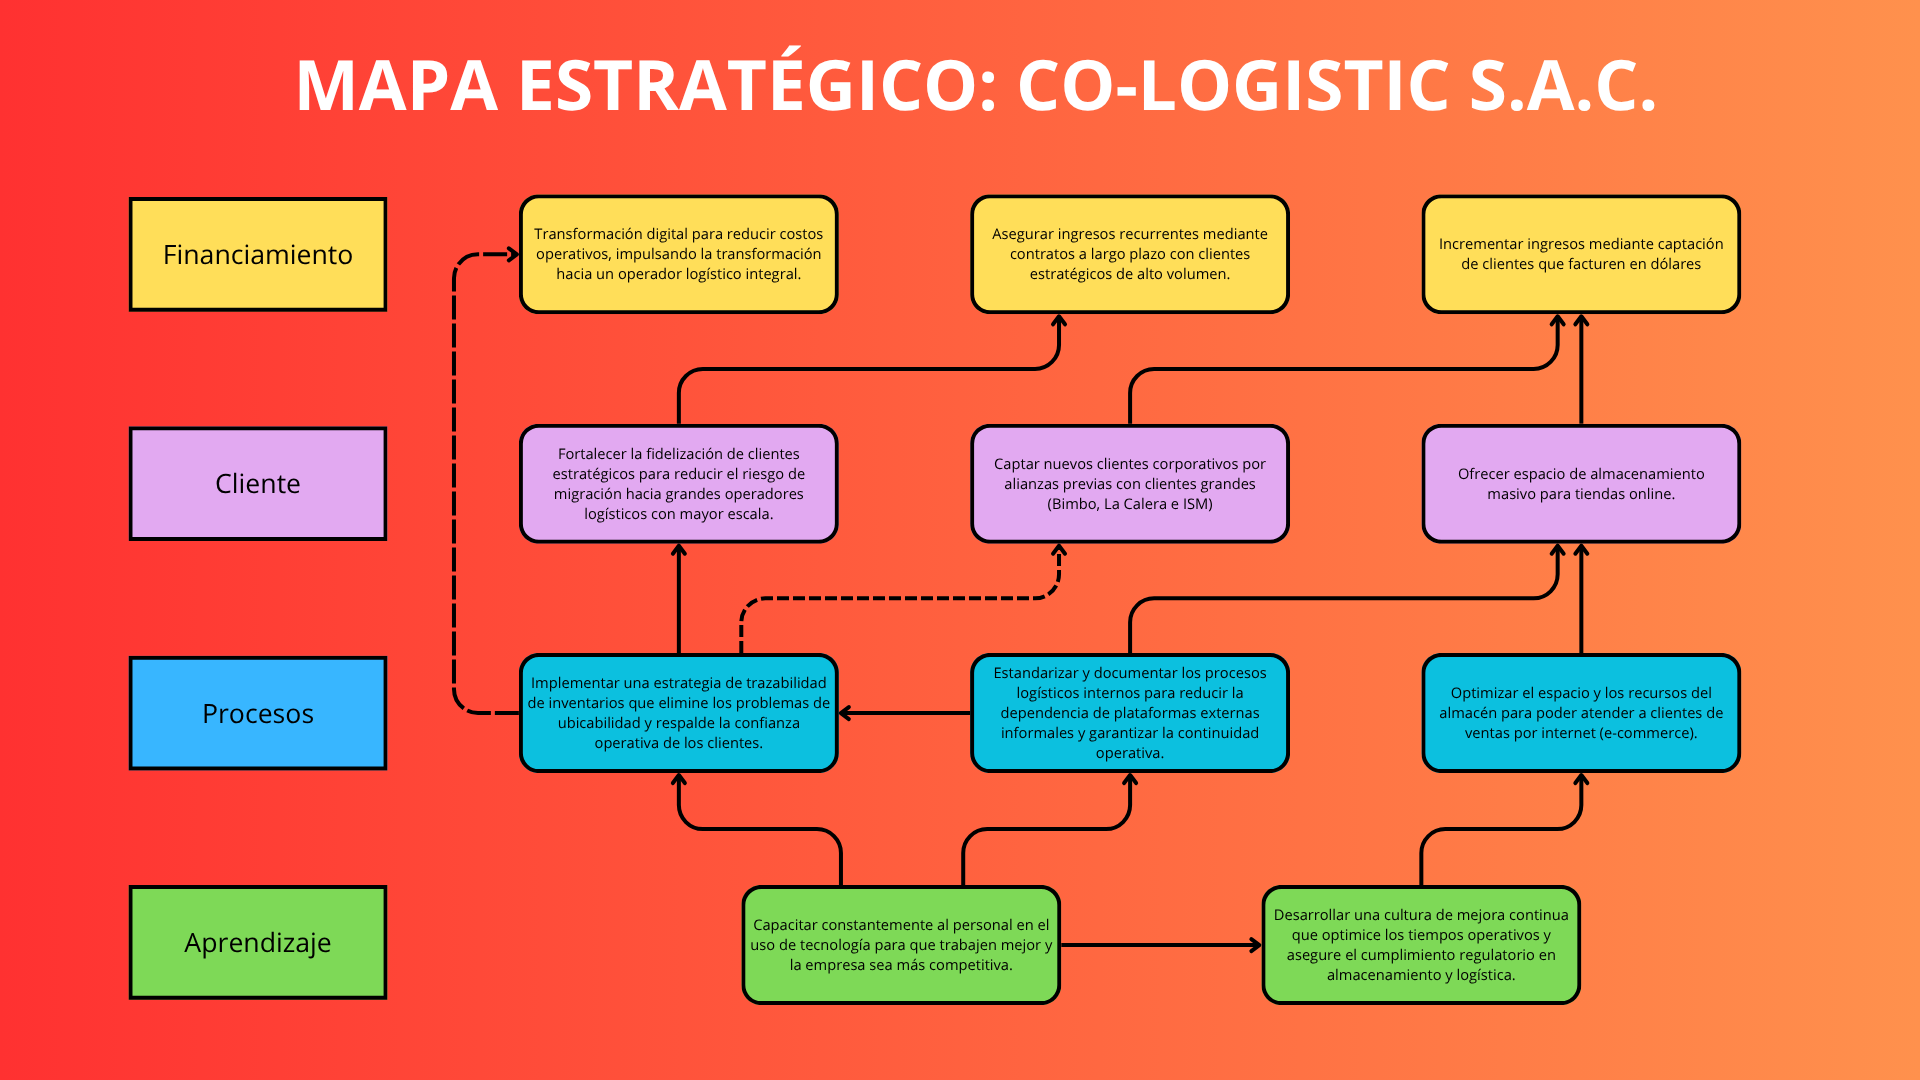
\includegraphics[width=5.5in,keepaspectratio]{media/image6.png}}
\end{center}

\vspace{0.3cm}
\setlength{\tabcolsep}{5pt}
\renewcommand{\arraystretch}{1.5}
\arrayrulecolor{TableLine}
{\def\LTcaptype{none}
\begin{longtable}[]{@{}
  >{\raggedright\arraybackslash}p{0.30\linewidth}
  >{\raggedright\arraybackslash}p{0.28\linewidth}
  >{\raggedright\arraybackslash}p{0.16\linewidth}
  >{\raggedright\arraybackslash}p{0.26\linewidth}@{}}
\rowcolor{DeepNavy}
\textcolor{white}{\textbf{Estrategia de negocio}} & \textcolor{white}{\textbf{Problema que atiende}} & \textcolor{white}{\textbf{Estrategia de TI}} & \textcolor{white}{\textbf{Aporte esperado}} \\ \hline
\endhead
\rowcolor{LightGray}
Implementar un sistema de trazabilidad de inventarios que elimine los problemas de ubicabilidad y respalde la confianza operativa de los clientes. & Dificultad para ubicar productos, errores de inventario, baja visibilidad operativa y riesgo de reclamos. & \multirow{2}{=}{Optimizar procesos logísticos con WMS/ERP en la nube.} & Permitir el registro, ubicación, consulta y seguimiento del inventario de forma centralizada y confiable. \\ \hline
Estandarizar y documentar los procesos logísticos internos para reducir la dependencia de plataformas externas informales y garantizar la continuidad operativa. & Procesos ejecutados de forma manual o informal, dependencia de Excel, falta de documentación aprobada y riesgo de interrupción operativa. & & Digitalizar procesos logísticos, documentar procedimientos, definir responsables y reducir la dependencia de herramientas no controladas. \\ \hline
\end{longtable}
}

\subsection*{Objetivo y Alcance del Plan}

\textbf{Objetivo del documento:} Establecer el plan de implementación del proceso APO02 --- Gestionar la Estrategia en CO LOGISTIC S.A.C., con la finalidad de formalizar la estrategia de TI ``Optimizar procesos logísticos con WMS/ERP en la nube'', alineándola con los objetivos del negocio, definiendo fases de ejecución, responsables, indicadores, riesgos, evidencias y mecanismos de mejora continua.

\textbf{Alcance del documento:}
* \textbf{Incluye:} Contexto actual de CO LOGISTIC S.A.C., relación entre estrategias de negocio y estrategia de TI, aplicación del proceso APO02 a la estrategia WMS/ERP en la nube, diagnóstico AS-IS resumido, estado futuro TO-BE, análisis de brechas, habilitadores COBIT adaptados al caso, fases de implementación, herramientas de soporte, KPIs principales, roadmap tecnológico resumido, riesgos estratégicos principales, matriz RACI preliminar, evidencias documentales y conclusiones.
* \textbf{No incluye:} Desarrollo completo de un software WMS/ERP propio, implementación técnica final de todos los módulos del sistema, compra definitiva de una solución tecnológica específica, contratación formal de proveedor, diseño detallado de infraestructura cloud, ni la configuración real de servidores, bases de datos o APIs.

---

\section{Fase 1: Preparación e Inicio del Proceso APO02}

\subsection{Propósito de la Fase}
La fase de preparación e inicio tiene como objetivo establecer las bases para aplicar APO02 en CO LOGISTIC S.A.C., identificando los impulsores estratégicos, el alcance del proceso, los objetivos SMART y los actores responsables de la estrategia de TI.

\subsection{Impulsores Específicos}
Los principales impulsores que justifican la implementación de APO02 son:
* Necesidad de mejorar la trazabilidad de inventarios.
* Problemas de ubicabilidad de productos dentro de los procesos logísticos.
* Dependencia de registros manuales, Excel o plataformas externas informales.
* Falta de procesos logísticos completamente documentados y estandarizados.
* Necesidad de continuidad operativa frente a cambios, rotación de personal o fallas de herramientas.
* Necesidad de alinear las iniciativas tecnológicas con los objetivos reales del negocio.
* Necesidad de contar con indicadores que permitan medir el avance y valor de las iniciativas de TI.
* Necesidad de evitar que futuras iniciativas tecnológicas queden inconclusas o sin seguimiento formal.

\subsection{Alcance del Proceso APO02}
El proceso APO02 se aplicará a la gestión de la estrategia de TI orientada a la optimización de procesos logísticos mediante un WMS/ERP en la nube. El alcance considera los siguientes elementos:
* Identificación de necesidades estratégicas del negocio.
* Alineamiento de la estrategia de TI con las estrategias del negocio.
* Diagnóstico de la situación actual.
* Definición del estado futuro.
* Elaboración del roadmap tecnológico.
* Definición de KPIs.
* Identificación de riesgos estratégicos.
* Asignación de responsables mediante matriz RACI.
* Seguimiento y mejora continua de la estrategia.

\subsection{Objetivos SMART}

\vspace{0.3cm}
\setlength{\tabcolsep}{6pt}
\renewcommand{\arraystretch}{1.5}
\arrayrulecolor{TableLine}
{\def\LTcaptype{none}
\begin{longtable}[]{@{}
  >{\centering\arraybackslash}p{0.18\linewidth}
  >{\raggedright\arraybackslash}p{0.82\linewidth}@{}}
\rowcolor{DeepNavy}
\textcolor{white}{\textbf{Criterio}} & \textcolor{white}{\textbf{Objetivo aplicado a CO LOGISTIC S.A.C.}} \\ \hline
\endhead
\rowcolor{LightGray}
\textbf{Específico} & Implementar un modelo de gestión estratégica de TI basado en APO02 para optimizar procesos logísticos mediante WMS/ERP en la nube. \\ \hline
\textbf{Medible} & Digitalizar al menos el 85\% de los procesos logísticos priorizados y alcanzar un 95\% de exactitud de inventario. \\ \hline
\rowcolor{LightGray}
\textbf{Alcanzable} & Utilizar información existente de la empresa, procesos actuales, documentos internos y herramientas cloud viables. \\ \hline
\textbf{Relevante} & Mejorar la trazabilidad, ubicabilidad, documentación de procesos, continuidad operativa y toma de decisiones. \\ \hline
\rowcolor{LightGray}
\textbf{Temporal} & Ejecutar el roadmap inicial en un periodo estimado de 12 meses. \\ \hline
\end{longtable}
}

\subsection{Mapa de Proceso}
\begin{center}
  \pandocbounded{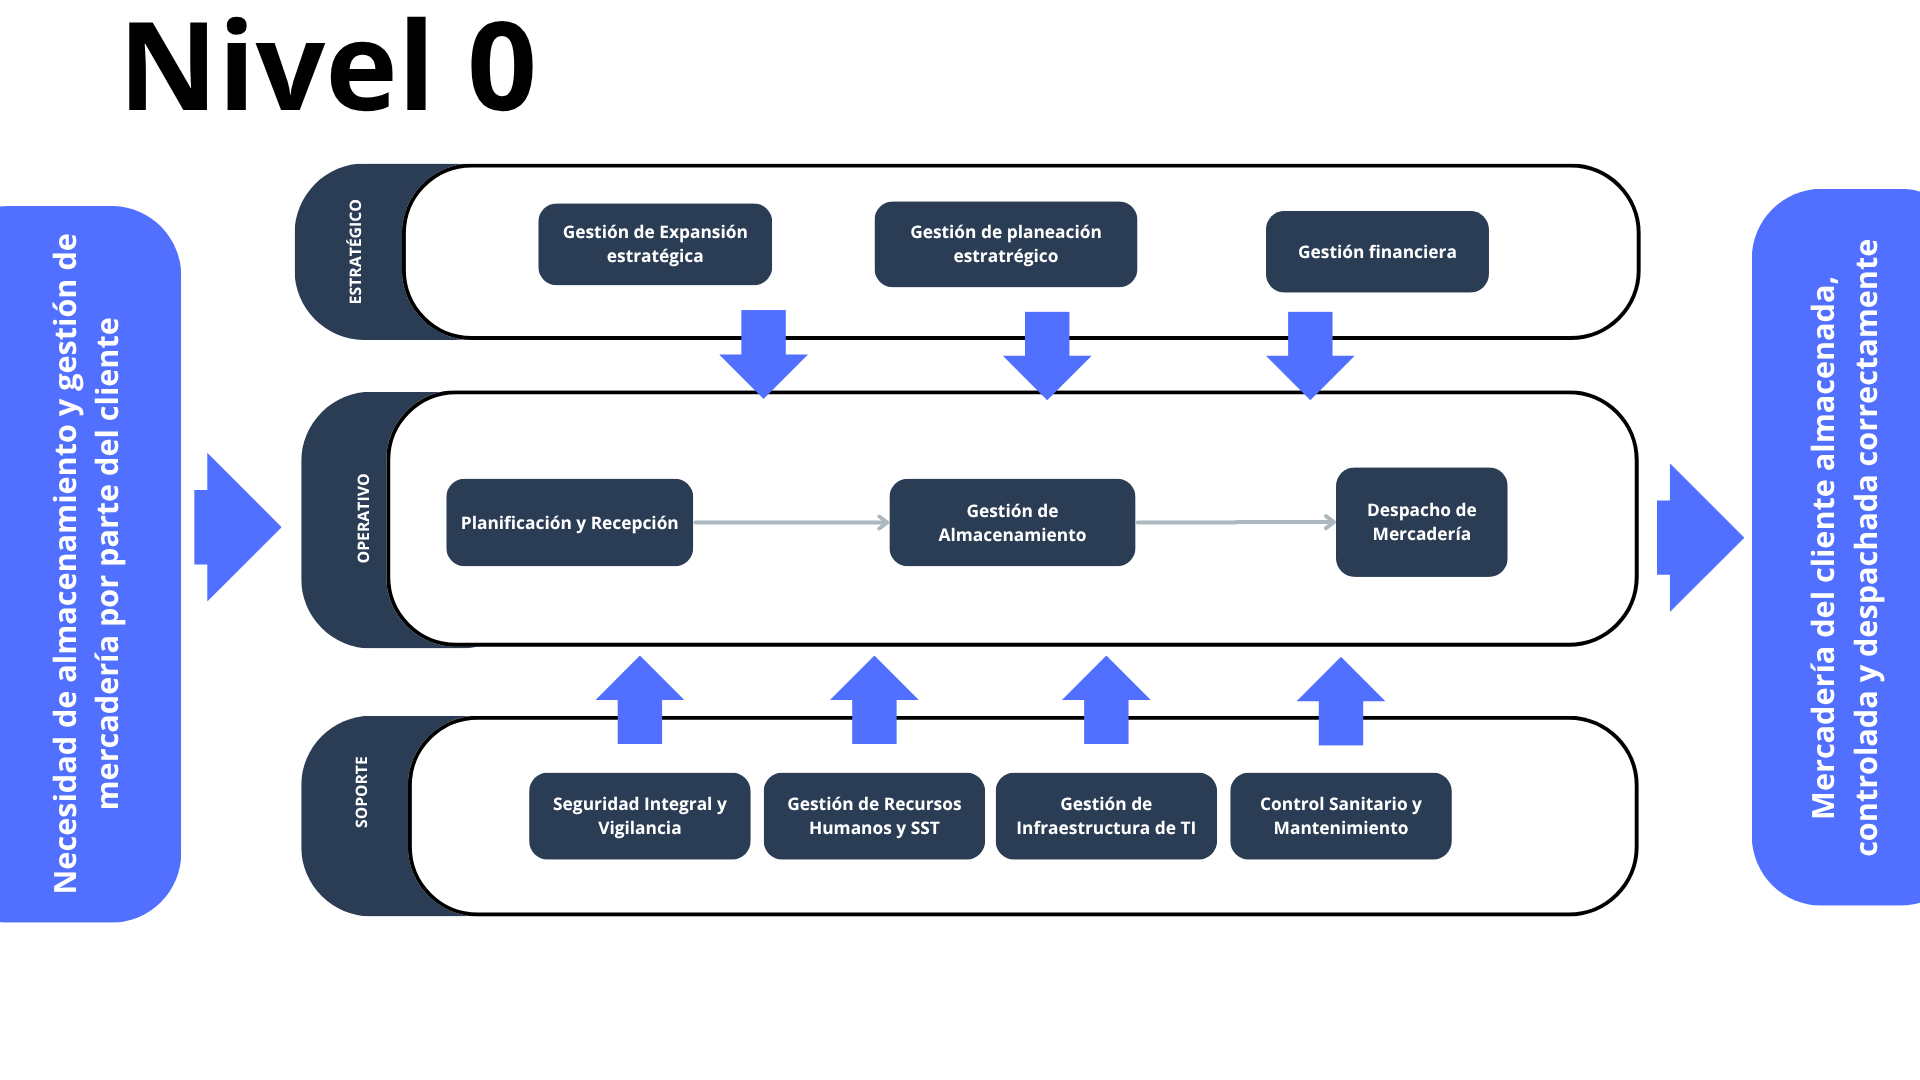
\includegraphics[width=6.5in,keepaspectratio]{media/image7.png}}
\end{center}

\subsection{Organigrama}
\begin{center}
  \pandocbounded{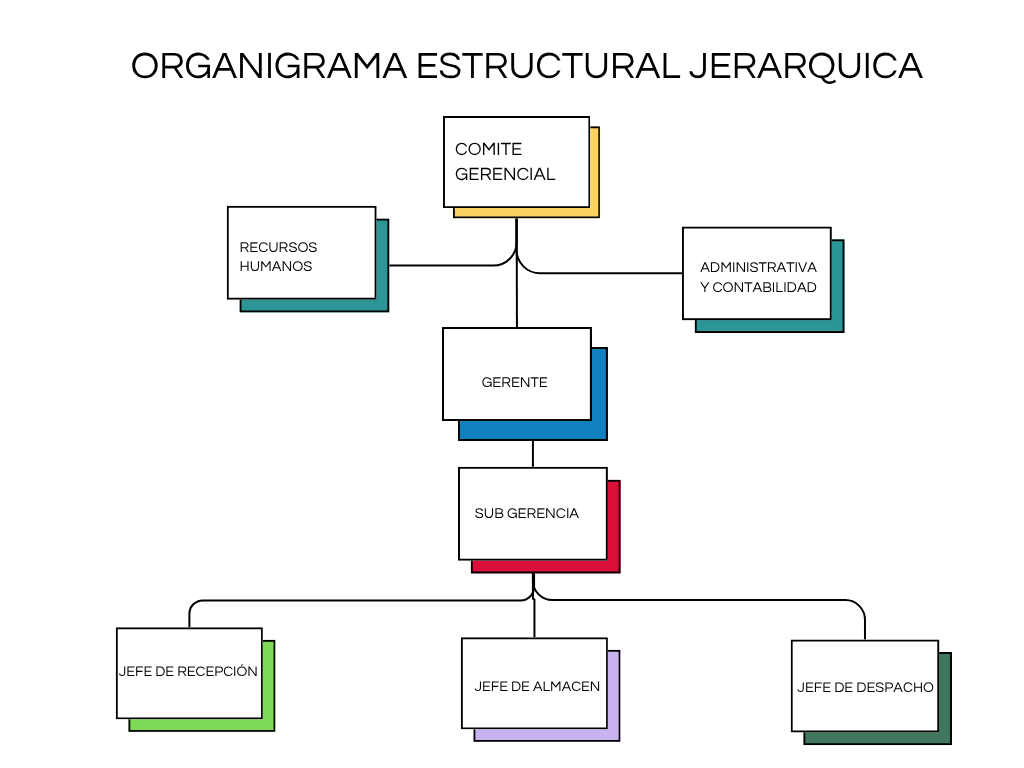
\includegraphics[width=5.5in,keepaspectratio]{media/image8.png}}
\end{center}

\subsection{Equipo de Implementación}
Para la ejecución exitosa del roadmap de TI y la adopción del proceso APO02 en CO LOGISTIC S.A.C., se ha conformado un equipo de implementación estratégico multidisciplinario, integrado por los siguientes profesionales responsables de asegurar la gobernanza, continuidad y valor de las iniciativas:

\vspace{0.3cm}
\setlength{\tabcolsep}{6pt}
\renewcommand{\arraystretch}{1.5}
\arrayrulecolor{TableLine}
{\def\LTcaptype{none}
\begin{longtable}[]{@{}
  >{\raggedright\arraybackslash}p{0.32\linewidth}
  >{\raggedright\arraybackslash}p{0.25\linewidth}
  >{\raggedright\arraybackslash}p{0.43\linewidth}@{}}
\rowcolor{DeepNavy}
\textcolor{white}{\textbf{Rol en el Proyecto}} & \textcolor{white}{\textbf{Responsable}} & \textcolor{white}{\textbf{Funciones Clave}} \\ \hline
\endhead
Director de Gobierno de TI / Patrocinador Principal & Abel Is-Boset Guevara Huasco & Liderar el comité estratégico de TI, autorizar presupuestos y asegurar la alineación entre la estrategia del negocio y de TI. \\ \hline
\rowcolor{LightGray}
Líder del Proyecto APO02 (APO02 Lead) & Jhack Ernesto Quispe Mamani & Planificar, coordinar y monitorear la implementación del roadmap estratégico, gestionando los scorecards y KPIs del BSC Designer. \\ \hline
Arquitecto de Soluciones WMS/ERP & Javier Kevin Tello Rivas & Diseñar la arquitectura técnica de la solución en la nube, coordinar la integración de datos y evaluar la viabilidad de proveedores. \\ \hline
\rowcolor{LightGray}
Analista de Procesos Logísticos & Richard Joseft Yanqui Inocente & Estandarizar y documentar los procesos logísticos operativos (TO-BE), asegurando su mapeo y correcta configuración en el WMS/ERP. \\ \hline
Especialista en Riesgos y Cumplimiento & Alvaro Kenji Cuti Magaño & Monitorear la matriz de riesgos estratégicos, definir planes de mitigación y asegurar la conformidad con regulaciones externas. \\ \hline
\rowcolor{LightGray}
Analista de Infraestructura y Soporte Cloud & David Guerra Ordoñez & Administrar el despliegue del WMS/ERP en la nube, garantizar la disponibilidad de la red y dar soporte de nivel tecnológico a la operación. \\ \hline
Gestor de Cambio y Capacitación & Joshua Alfonzo Javier & Diseñar e implementar el plan de comunicación, mitigar la resistencia al cambio de los usuarios y dictar talleres sobre las nuevas herramientas. \\ \hline
\rowcolor{LightGray}
Especialista en QA e Integración & Sebastían Chinchay Collachagua & Validar la calidad del sistema, ejecutar las pruebas de control de inventarios y coordinar interfaces con otros sistemas de soporte. \\ \hline
\end{longtable}
}

---

\section{Fase 2: Evaluación y Diseño Detallado del Proceso APO02}

\subsection{Propósito de la Fase}
Esta fase tiene como finalidad analizar la situación actual de CO LOGISTIC S.A.C., identificar brechas frente al estado deseado y diseñar el modelo de gestión estratégica de TI basado en APO02.

\subsection{Análisis FODA}
*(Se integra en la matriz PESTEL y de riesgos estratégicos de la organización).*

\subsection{Evaluación del Estado Actual (AS-IS)}
Actualmente, CO LOGISTIC S.A.C. presenta una gestión logística con oportunidades de mejora en trazabilidad, ubicabilidad y estandarización documental. Parte del control operativo se apoya en registros manuales, archivos de Excel o herramientas no completamente integradas, lo cual puede generar duplicidad de información, errores de registro, dificultad para ubicar productos, pérdida de trazabilidad y dependencia del conocimiento operativo de determinadas personas.

Asimismo, la empresa cuenta con iniciativas estratégicas orientadas a mejorar su operación, pero requiere fortalecer el seguimiento formal de dichas iniciativas mediante responsables, indicadores, roadmap, riesgos y evidencias de avance. Esta situación evidencia la necesidad de implementar un modelo de gestión estratégica de TI que permita priorizar, controlar y medir las iniciativas tecnológicas con impacto directo en el negocio.

\subsubsection{Análisis de Brecha (GAP)}

\vspace{0.3cm}
\setlength{\tabcolsep}{5pt}
\renewcommand{\arraystretch}{1.5}
\arrayrulecolor{TableLine}
{\def\LTcaptype{none}
\begin{longtable}[]{@{}
  >{\raggedright\arraybackslash}p{0.30\linewidth}
  >{\raggedright\arraybackslash}p{0.28\linewidth}
  >{\raggedright\arraybackslash}p{0.42\linewidth}@{}}
\rowcolor{DeepNavy}
\textcolor{white}{\textbf{Situación actual}} & \textcolor{white}{\textbf{Brecha identificada}} & \textcolor{white}{\textbf{Situación esperada con APO02 y WMS/ERP}} \\ \hline
\endhead
\rowcolor{LightGray}
Inventarios controlados mediante registros manuales o Excel. & Falta de sistema centralizado para trazabilidad. & Inventarios gestionados mediante WMS/ERP en la nube. \\ \hline
Procesos logísticos no completamente documentados. & Falta de documentación formal y control de versiones. & Procesos logísticos estandarizados, aprobados y controlados. \\ \hline
\rowcolor{LightGray}
Dificultad para ubicar productos. & Problemas de ubicabilidad y control físico-lógico. & Ubicación exacta y actualizada de productos en el sistema. \\ \hline
Uso de herramientas informales o dispersas. & Información fragmentada y bajo control institucional. & Ecosistema integrado con WMS/ERP, dashboard y repositorio documental. \\ \hline
\rowcolor{LightGray}
Decisiones operativas con baja medición. & Falta de indicadores consolidados. & Toma de decisiones basada en KPIs y reportes. \\ \hline
Iniciativas TI sin seguimiento estratégico completo. & Falta de gobierno formal sobre la estrategia TI. & Iniciativas priorizadas, monitoreadas y evaluadas bajo APO02. \\ \hline
\end{longtable}
}

\subsubsection{Situación Actual (AS-IS)}

\vspace{0.3cm}
\setlength{\tabcolsep}{5pt}
\renewcommand{\arraystretch}{1.5}
\arrayrulecolor{TableLine}
{\def\LTcaptype{none}
\begin{longtable}[]{@{}
  >{\raggedright\arraybackslash}p{0.46\linewidth}
  >{\centering\arraybackslash}p{0.18\linewidth}
  >{\centering\arraybackslash}p{0.18\linewidth}
  >{\centering\arraybackslash}p{0.18\linewidth}@{}}
\rowcolor{DeepNavy}
\textcolor{white}{\textbf{Componente APO02}} & \textcolor{white}{\textbf{Nivel actual}} & \textcolor{white}{\textbf{Nivel objetivo}} & \textcolor{white}{\textbf{GAP}} \\ \hline
\endhead
\rowcolor{LightGray}
Alineación negocio--TI & 2 & 4 & 2 \\ \hline
Definición de estrategia TI & 2 & 4 & 2 \\ \hline
\rowcolor{LightGray}
Documentación de estrategia & 2 & 4 & 2 \\ \hline
Comunicación de estrategia & 1 & 3 & 2 \\ \hline
\rowcolor{LightGray}
Roadmap de TI & 1 & 4 & 3 \\ \hline
Portafolio de iniciativas & 1 & 4 & 3 \\ \hline
\rowcolor{LightGray}
KPIs estratégicos & 1 & 4 & 3 \\ \hline
Seguimiento y control & 1 & 4 & 3 \\ \hline
\rowcolor{LightGray}
Analítica y apoyo a decisiones & 0 & 4 & 4 \\ \hline
Mejora continua y evolución tecnológica & 1 & 5 & 4 \\ \hline
\end{longtable}
}

\subsubsection{Evaluación de la Capacidad}

\vspace{0.3cm}
\setlength{\tabcolsep}{5pt}
\renewcommand{\arraystretch}{1.5}
\arrayrulecolor{TableLine}
{\def\LTcaptype{none}
\begin{longtable}[]{@{}
  >{\centering\arraybackslash}p{0.22\linewidth}
  >{\centering\arraybackslash}p{0.12\linewidth}
  >{\centering\arraybackslash}p{0.12\linewidth}
  >{\centering\arraybackslash}p{0.08\linewidth}
  >{\raggedright\arraybackslash}p{0.46\linewidth}@{}}
\rowcolor{DeepNavy}
\textcolor{white}{\textbf{Componente APO02}} & \textcolor{white}{\textbf{Nivel Act.}} & \textcolor{white}{\textbf{Nivel Obj.}} & \textcolor{white}{\textbf{GAP}} & \textcolor{white}{\textbf{Brechas Identificadas}} \\ \hline
\endhead
\rowcolor{LightGray}
Alineación negocio--TI & 2 & 4 & 2 & La estrategia tecnológica aún no se encuentra completamente alineada a los procesos operativos y logísticos de la organización. \\ \hline
Definición de estrategia TI & 2 & 4 & 2 & No existe una estrategia tecnológica formalmente integrada con objetivos medibles y evolución digital definida. \\ \hline
\rowcolor{LightGray}
Documentación de estrategia & 2 & 4 & 2 & La documentación estratégica aún presenta dispersión documental y ausencia de control centralizado y versionamiento formal. \\ \hline
Comunicación de estrategia & 1 & 3 & 2 & La comunicación estratégica depende principalmente de reuniones informales y no existen mecanismos estructurados de difusión y seguimiento. \\ \hline
\rowcolor{LightGray}
Roadmap de TI & 1 & 4 & 3 & La organización no dispone de una hoja de ruta tecnológica formal que permita planificar la evolución digital y operativa del negocio. \\ \hline
Portafolio de iniciativas & 1 & 4 & 3 & Las iniciativas estratégicas no cuentan con priorización, seguimiento ni evaluación continua mediante herramientas centralizadas. \\ \hline
\rowcolor{LightGray}
KPIs estratégicos & 1 & 4 & 3 & No existen indicadores automatizados que permitan medir el desempeño logístico y operativo en tiempo real. \\ \hline
Seguimiento y control & 1 & 4 & 3 & El monitoreo de procesos y actividades se realiza de manera manual mediante hojas de cálculo y supervisión operativa básica. \\ \hline
\rowcolor{LightGray}
Analítica y apoyo a decisiones & 0 & 4 & 4 & La organización no cuenta con herramientas analíticas ni capacidades de inteligencia de negocio para apoyar la toma de decisiones estratégicas. \\ \hline
Mejora continua y evolución tecnológica & 1 & 5 & 4 & No existe un modelo formal de innovación, retroalimentación organizacional y mejora tecnológica continua. \\ \hline
\end{longtable}
}

\subsubsection{Causas del GAP}

\vspace{0.3cm}
\setlength{\tabcolsep}{6pt}
\renewcommand{\arraystretch}{1.5}
\arrayrulecolor{TableLine}
{\def\LTcaptype{none}
\begin{longtable}[]{@{}
  >{\raggedright\arraybackslash}p{0.25\linewidth}
  >{\raggedright\arraybackslash}p{0.75\linewidth}@{}}
\rowcolor{DeepNavy}
\textcolor{white}{\textbf{Área del GAP}} & \textcolor{white}{\textbf{Causa Raíz Identificada}} \\ \hline
\endhead
\rowcolor{LightGray}
Roadmap & La estrategia organizacional no fue traducida en un plan tecnológico estructurado y evolutivo. \\ \hline
KPIs & La organización no posee cultura de medición ni herramientas automatizadas de monitoreo operacional. \\ \hline
\rowcolor{LightGray}
Seguimiento y control & Los procesos dependen de supervisión manual y no existe una plataforma centralizada de control y trazabilidad. \\ \hline
Comunicación estratégica & No existen mecanismos formales para difundir, monitorear y alinear los objetivos estratégicos organizacionales. \\ \hline
\rowcolor{LightGray}
Portafolio de iniciativas & Las iniciativas se gestionan de manera reactiva sin priorización basada en indicadores y objetivos estratégicos. \\ \hline
Analítica y toma de decisiones & La empresa no cuenta con herramientas de inteligencia de negocio ni análisis de datos para soporte gerencial. \\ \hline
\rowcolor{LightGray}
Mejora continua & No existe un mecanismo estructurado para recopilar retroalimentación, evaluar desempeño y evolucionar procesos y tecnología. \\ \hline
\end{longtable}
}

\subsubsection{Diagrama de Proceso AS-IS}

En la situación actual (AS-IS), CO LOGISTIC S.A.C. presenta flujos de trabajo altamente fragmentados y dependientes de la supervisión directa. Las decisiones estratégicas de TI no se documentan, los proyectos operan de manera aislada y el flujo de información carece de una plataforma centralizada de control, lo que se ilustra en el siguiente diagrama operativo:

\begin{itemize}
\item \textbf{Entradas:} Las iniciativas TI nacen por presión o urgencia del negocio, no por planificación estratégica.
\item \textbf{Reuniones ad-hoc:} Las decisiones se toman en reuniones informales o según lo que surge, sin una frecuencia definida ni seguimiento estructurado.
\item \textbf{Decisiones no trazables:} No hay registro ni justificación clara de por qué se hacen ciertas acciones o se priorizan algunos proyectos.
\item \textbf{Proyectos dispersos:} Cada iniciativa funciona aislada, sin un plan global, sin indicadores, sin revisión formal de resultados.
\end{itemize}

\begin{center}
  \pandocbounded{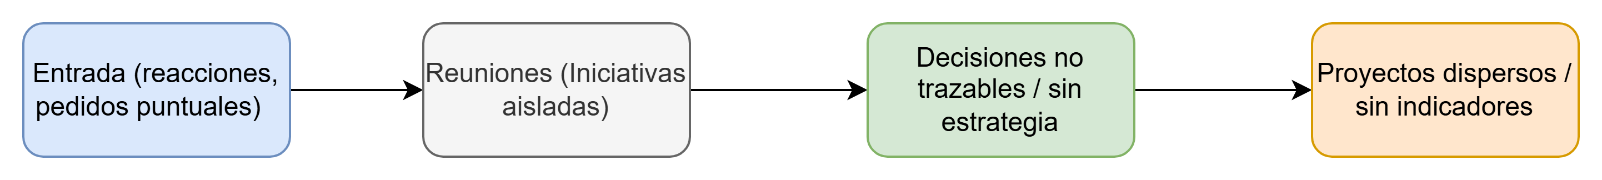
\includegraphics[width=6.5in,keepaspectratio]{media/image2.png}}
\end{center}

\subsection{Diseño del Estado Futuro (TO-BE)}
En el estado futuro, CO LOGISTIC S.A.C. contará con una estrategia de TI formalmente gestionada bajo el proceso APO02. Esta estrategia permitirá implementar progresivamente un WMS/ERP en la nube para digitalizar procesos logísticos, mejorar la trazabilidad de inventarios, controlar la ubicabilidad de productos y reducir la dependencia de herramientas informales.

Los procesos logísticos estarán documentados, los responsables serán definidos mediante una matriz RACI, los riesgos estratégicos serán monitoreados, los indicadores serán actualizados periódicamente y el roadmap tecnológico será revisado por un comité de seguimiento. De esta manera, la empresa podrá tomar decisiones basadas en información confiable y asegurar que la tecnología genere valor real para el negocio.

\subsubsection{Nivel de Capacidad Objetivo}

\vspace{0.3cm}
\setlength{\tabcolsep}{5pt}
\renewcommand{\arraystretch}{1.5}
\arrayrulecolor{TableLine}
{\def\LTcaptype{none}
\begin{longtable}[]{@{}
  >{\raggedright\arraybackslash}p{0.24\linewidth}
  >{\raggedright\arraybackslash}p{0.56\linewidth}
  >{\centering\arraybackslash}p{0.20\linewidth}@{}}
\rowcolor{DeepNavy}
\textcolor{white}{\textbf{GAP}} & \textcolor{white}{\textbf{Acción recomendada}} & \textcolor{white}{\textbf{Prioridad (1-10)}} \\ \hline
\endhead
\rowcolor{LightGray}
Roadmap de TI & Elaborar un roadmap estratégico y tecnológico alineando a los objetivos del negocio & 6 \\ \hline
KPIs & Definir indicadores operativos y estratégicos para monitoreo logístico y gerencial & 1 \\ \hline
\rowcolor{LightGray}
Seguimiento manual & Implementar dashboard para monitoreo logístico y gerencial & 2 \\ \hline
Baja analítica & Desarrollar herramientas de analítica y visualización para apoyo gerencial & 3 \\ \hline
\rowcolor{LightGray}
Comunicación limitada & Formalizar mecanismos de comunicación y seguimiento estratégico organizacional & 8 \\ \hline
Portafolio no priorizado & Implementar gestión centralizada y priorización de iniciativas estratégicas & 7 \\ \hline
\rowcolor{LightGray}
Falta de control & Automatizar procesos de control operativo mediante el sistema propuesto & 4 \\ \hline
Ausencia de mejora continua & Establecer backlog evolutivo y plan de mejora continua tecnológica & 9 \\ \hline
\rowcolor{LightGray}
Dependencia de manuales & Digitalizar y centralizar procesos logísticos y documentales & 5 \\ \hline
Escasa innovación & Incorporar funcionalidades de dashboard inteligente y analítica basada en IA & 10 \\ \hline
\end{longtable}
}

\subsection{Adaptación de Prácticas COBIT a CO LOGISTIC S.A.C.}

\textbf{- Habilitador 1: Principios, Políticas y Marcos}
Establece los lineamientos y reglas de juego del proceso. Para CO LOGISTIC S.A.C., se crea la \textbf{Política de Gobierno Estratégico de TI}, el uso de marcos metodológicos estructurados como COBIT y el Balanced Scorecard (BSC), y los Procedimientos Operativos Estandarizados (POEs) para regular las sesiones del comité.

\textbf{- Habilitador 2: Procesos (Flujo de Gestión y Adopción WMS/ERP)}
El habilitador de procesos garantiza que las actividades de la organización sigan un flujo estructurado y repetible. Para CO LOGISTIC S.A.C., el proceso APO02 se compone de un conjunto de prácticas integradas (comprensión de metas, evaluación AS-IS, diseño TO-BE, roadmap y KPIs) que aseguran que la adopción del software WMS/ERP en la nube esté debidamente orquestada, con entradas y salidas de información automatizadas que evitan los silos de datos y aseguran la trazabilidad de extremo a extremo.

\textbf{- Habilitador 3: Estructuras Organizacionales (Matriz RACI)}
Para delimitar con precisión la responsabilidad en la toma de decisiones y ejecución de cada práctica del proceso APO02 --- Gestionar la Estrategia, se ha definido la siguiente Matriz RACI:

\vspace{0.3cm}
\setlength{\tabcolsep}{5pt}
\renewcommand{\arraystretch}{1.5}
\arrayrulecolor{TableLine}
{\def\LTcaptype{none}
\begin{longtable}[]{@{}
  >{\raggedright\arraybackslash}p{0.38\linewidth}
  >{\centering\arraybackslash}p{0.10\linewidth}
  >{\centering\arraybackslash}p{0.10\linewidth}
  >{\centering\arraybackslash}p{0.10\linewidth}
  >{\centering\arraybackslash}p{0.10\linewidth}
  >{\centering\arraybackslash}p{0.10\linewidth}@{}}
\rowcolor{DeepNavy}
\textcolor{white}{\textbf{Prácticas del Proceso APO02}} & \textcolor{white}{\textbf{GG}} & \textcolor{white}{\textbf{CIO}} & \textcolor{white}{\textbf{ASC}} & \textcolor{white}{\textbf{APL}} & \textcolor{white}{\textbf{GCA}} \\ \hline
\endhead
\textbf{APO02.01: Comprender la dirección estratégica del negocio} & A & R & C & C & I \\ \hline
\rowcolor{LightGray}
\textbf{APO02.02: Evaluar entorno, capacidades y rendimiento de TI} & I & A & R & R & C \\ \hline
\textbf{APO02.03: Definir el estado futuro y capacidades de TI objetivo} & A & R & R & C & I \\ \hline
\rowcolor{LightGray}
\textbf{APO02.04: Realizar el análisis de brechas (GAP Analysis)} & I & A & R & R & C \\ \hline
\textbf{APO02.05: Elaborar el Plan Estratégico y Roadmap tecnológico} & A & R & R & C & C \\ \hline
\end{longtable}
}

\textbf{- Habilitador 4: Cultura, Ética y Comportamiento}
Actualmente, en CO LOGISTIC S.A.C. la cultura de trabajo se encuentra orientada principalmente a resolver las operaciones del día a día, apoyándose en registros manuales, Excel o herramientas informales para controlar inventarios, ubicaciones y procesos logísticos. Esto demuestra compromiso operativo del personal, pero también evidencia una cultura todavía poco estandarizada en cuanto al uso de información, trazabilidad, documentación formal y toma de decisiones basada en datos. Desde el aspecto ético, la empresa debe fortalecer la responsabilidad en el registro correcto de la información, ya que un dato incompleto o mal ingresado puede afectar la confianza operativa, la continuidad del servicio y la relación con los clientes.

Con la implementación de APO02 y la estrategia de TI \textbf{``Optimizar procesos logísticos con WMS/ERP en la nube''}, CO LOGISTIC busca avanzar hacia una cultura organizacional más ordenada, trazable y orientada a objetivos estratégicos. El comportamiento esperado es que el personal use el WMS/ERP como fuente oficial de información, registre los datos de manera correcta, respete los procesos documentados y participe activamente en la mejora continua. Además, se busca fomentar la toma de decisiones basada en indicadores, campañas internas de alineación estratégica, capacitaciones y una conducta ética enfocada en la confidencialidad, exactitud y uso responsable de la información logística.

\textbf{- Habilitador 5: Información (Matriz de Análisis PESTEL)}

\vspace{0.3cm}
\setlength{\tabcolsep}{5pt}
\renewcommand{\arraystretch}{1.5}
\arrayrulecolor{TableLine}
{\def\LTcaptype{none}
\begin{longtable}[]{@{}
  >{\raggedright\arraybackslash}p{0.14\linewidth}
  >{\raggedright\arraybackslash}p{0.62\linewidth}
  >{\centering\arraybackslash}p{0.12\linewidth}
  >{\centering\arraybackslash}p{0.12\linewidth}@{}}
\rowcolor{DeepNavy}
\textcolor{white}{\textbf{Dimensión}} & \textcolor{white}{\textbf{Factor PESTEL Analizado}} & \textcolor{white}{\textbf{Amenaza}} & \textcolor{white}{\textbf{Oport.}} \\ \hline
\endhead
\multirow{7}{=}{\textbf{POLÍTICO}} & Gobierno de turno (inestabilidad política y regulatoria). & X & \\ \cline{2-4}
& Alejamiento de clientes extranjeros por inestabilidad del país. & X & \\ \cline{2-4}
& Políticas que favorecen a la digitalización de las MYPEs. & & X \\ \cline{2-4}
& Gestión y trámites con sectores públicos. & X & \\ \cline{2-4}
& Inestabilidad en la seguridad del transporte terrestre nacional. & X & \\ \cline{2-4}
& Inacción en seguridad ciudadana (extorsión comercial). & X & \\ \cline{2-4}
& Relación ágil con entidades públicas de control (SUNAT). & & X \\ \hline
\rowcolor{LightGray}
\multirow{6}{=}{\textbf{ECONÓMICO}} & Alza del tipo de cambio del Dólar (afecta licenciamiento cloud). & X & \\ \cline{2-4}
\rowcolor{LightGray}
& Alza del precio de alquiler de locales para almacenes. & X & \\ \cline{2-4}
\rowcolor{LightGray}
& Alta informalidad del sector que genera competencia desleal. & X & \\ \cline{2-4}
\rowcolor{LightGray}
& Inflación generalizada y alza de combustibles. & X & \\ \cline{2-4}
\rowcolor{LightGray}
& Crecimiento del comercio electrónico (e-commerce) en el país. & & X \\ \cline{2-4}
\rowcolor{LightGray}
& Competencia con grandes operadores logísticos. & X & \\ \hline
\multirow{5}{=}{\textbf{SOCIAL}} & Inseguridad ciudadana y robos en locales logísticos. & X & \\ \cline{2-4}
& Escasez de talento humano logístico calificado. & X & \\ \cline{2-4}
& Cultura organizacional resistente a herramientas tecnológicas. & X & \\ \cline{2-4}
& Conflictos sociales, paros y protestas en vías de transporte. & X & \\ \cline{2-4}
& Incremento de la confianza del cliente en la trazabilidad digital. & & X \\ \hline
\rowcolor{LightGray}
\multirow{5}{=}{\textbf{TECNOLÓGICO}} & IoT en la cadena de suministro (trazabilidad física). & & X \\ \cline{2-4}
\rowcolor{LightGray}
& Dependencia de licencias tradicionales de software de oficina. & X & \\ \cline{2-4}
\rowcolor{LightGray}
& Disponibilidad de red de conectividad 5G y fibra óptica local. & & X \\ \cline{2-4}
\rowcolor{LightGray}
& Caídas temporales de servidores o redes en la nube. & X & \\ \cline{2-4}
\rowcolor{LightGray}
& Mercado de software WMS/ERP escalable como servicio (SaaS). & & X \\ \hline
\multirow{5}{=}{\textbf{ECOLÓGICO}} & Presión para reducción del uso de papel en almacén. & & X \\ \cline{2-4}
& Normativas sobre manejo y almacenamiento de residuos. & & X \\ \cline{2-4}
& Exposición de almacenes a lluvias intensas (Fenómeno El Niño). & X & \\ \cline{2-4}
& Restricciones de almacenamiento de productos químicos. & X & \\ \cline{2-4}
& Campañas de reciclaje y optimización de cartones y palets. & & X \\ \hline
\rowcolor{LightGray}
\multirow{4}{=}{\textbf{LEGAL}} & Regulaciones de guías de remisión electrónicas (SUNAT). & X & X \\ \cline{2-4}
\rowcolor{LightGray}
& Leyes de seguridad ocupacional y salud en el trabajo (SST). & X & \\ \cline{2-4}
\rowcolor{LightGray}
& Normativas municipales de almacenamiento y zonificación. & X & \\ \cline{2-4}
\rowcolor{LightGray}
& Formalización contractual de responsabilidades de carga. & & X \\ \hline
\end{longtable}
}

\vspace{0.4cm}
\textbf{Mapa de Estrategia del negocio:}
\begin{center}
  \pandocbounded{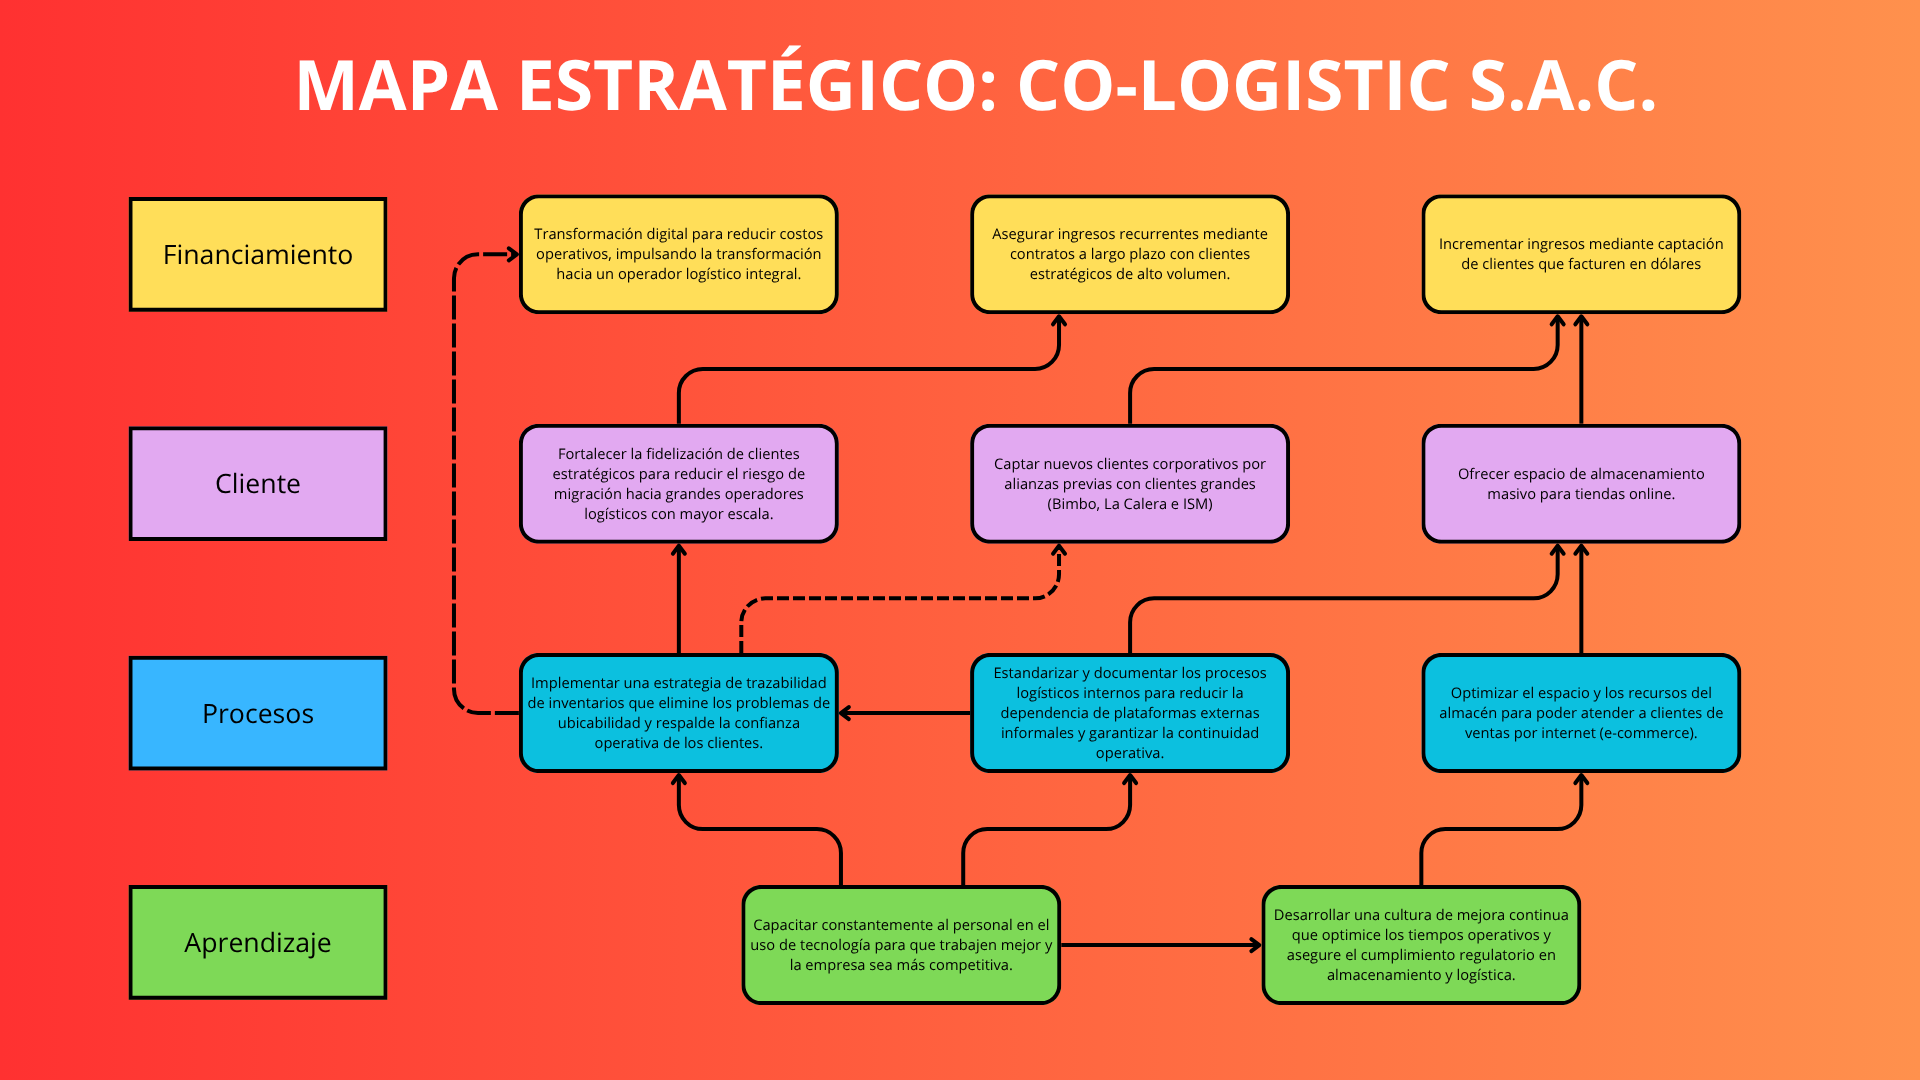
\includegraphics[width=6.5in,keepaspectratio]{media/image9.png}}
\end{center}

\textbf{Mapa de Estrategia de TI:}
\begin{center}
  \pandocbounded{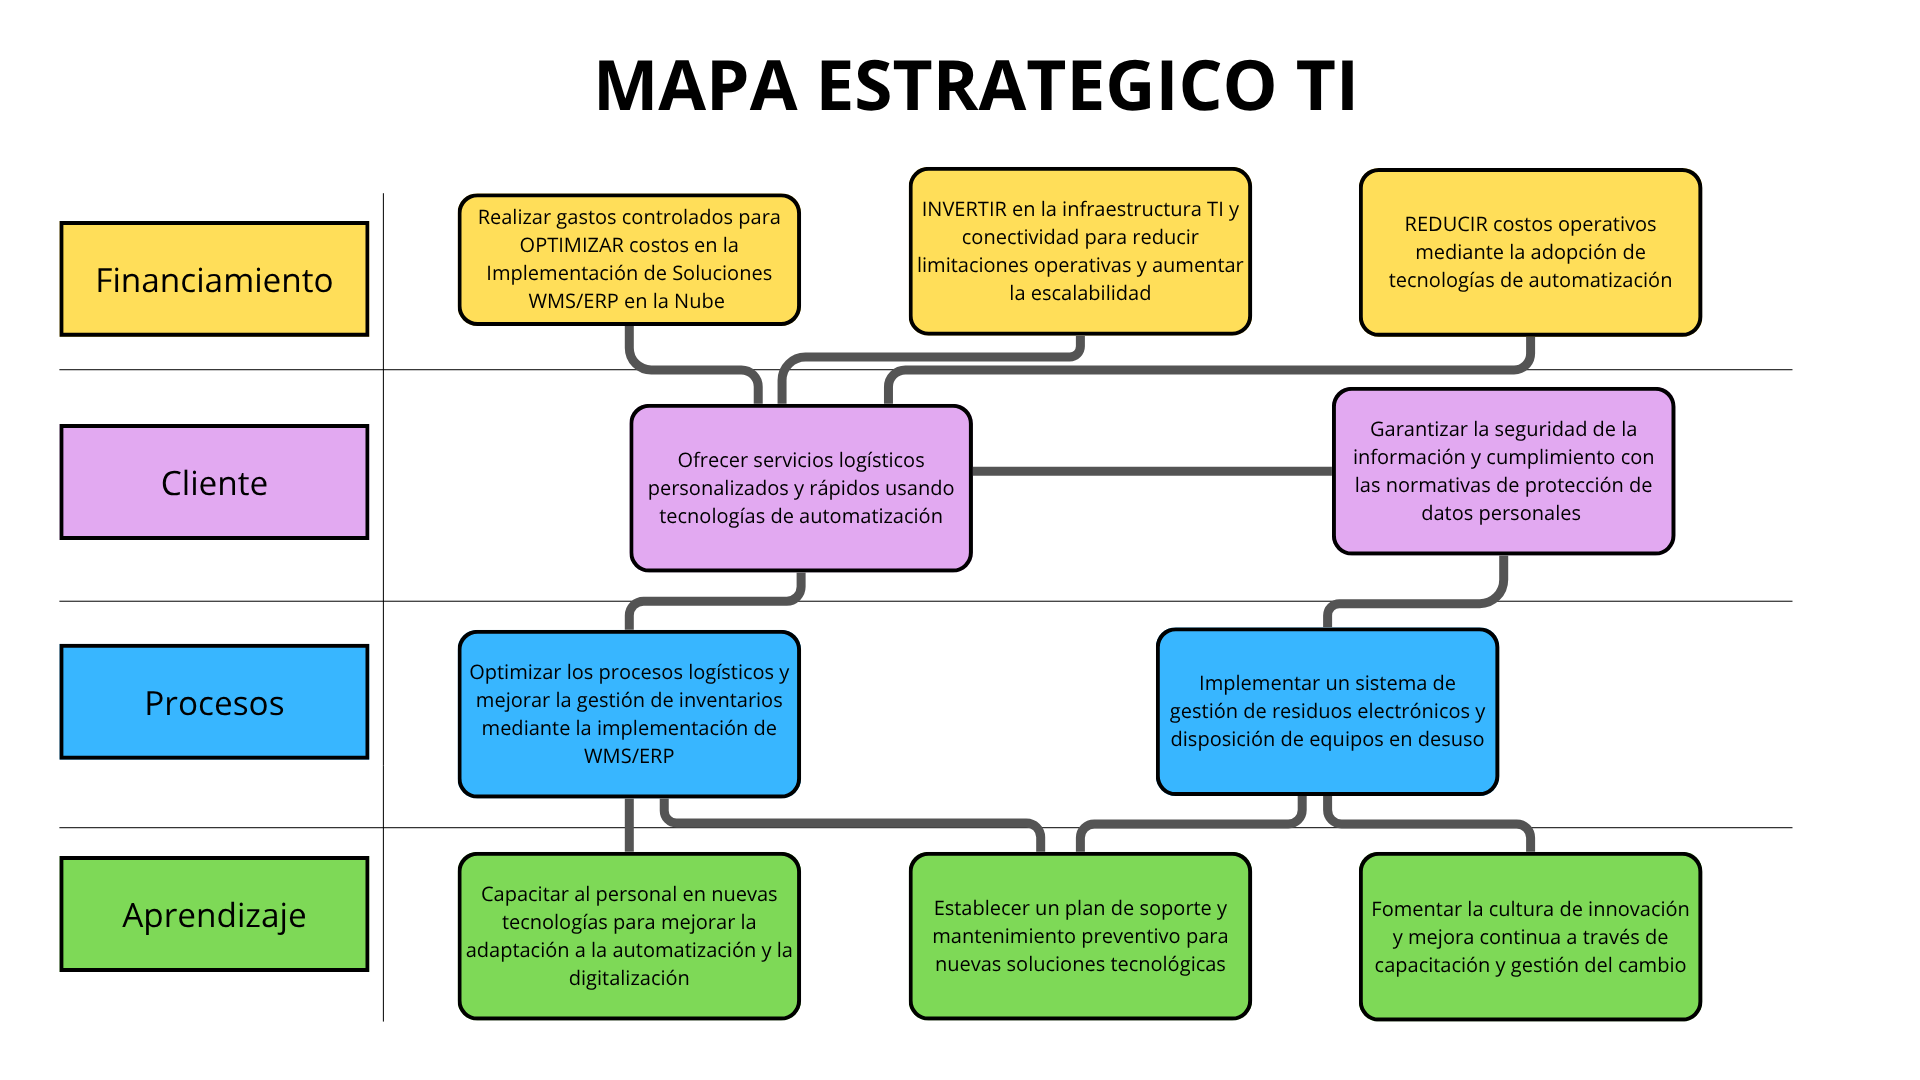
\includegraphics[width=6.5in,keepaspectratio]{media/imagea.png}}
\end{center}

\textbf{Matriz de riesgo estratégico:}
Para garantizar que la transición al modelo de TI basado en APO02 y el despliegue del WMS/ERP en la nube sean exitosos, se ha diseñado una Matriz de Riesgo Estratégico. Esta matriz identifica las principales amenazas, su nivel de criticidad (determinado por el producto de la Probabilidad e Impacto, en escala del 1 al 5) y las respectivas estrategias de mitigación formuladas:

\vspace{0.3cm}
\setlength{\tabcolsep}{5pt}
\renewcommand{\arraystretch}{1.5}
\arrayrulecolor{TableLine}
{\def\LTcaptype{none}
\begin{longtable}[]{@{}
  >{\raggedright\arraybackslash}p{0.30\linewidth}
  >{\centering\arraybackslash}p{0.08\linewidth}
  >{\centering\arraybackslash}p{0.08\linewidth}
  >{\centering\arraybackslash}p{0.12\linewidth}
  >{\raggedright\arraybackslash}p{0.42\linewidth}@{}}
\rowcolor{DeepNavy}
\textcolor{white}{\textbf{Riesgo Estratégico}} & \textcolor{white}{\textbf{Prob.}} & \textcolor{white}{\textbf{Imp.}} & \textcolor{white}{\textbf{Severidad}} & \textcolor{white}{\textbf{Estrategia de Mitigación y Control}} \\ \hline
\endhead
\textbf{Resistencia cultural al cambio} por parte del personal operativo de almacén ante el WMS/ERP. & 4 & 4 & \textbf{\color{red}16 (Alto)} & Ejecutar el Plan de Gestión del Cambio, realizar talleres participativos e incentivar el uso de la herramienta mediante gamificación. \\ \hline
\rowcolor{LightGray}
\textbf{Interrupción de la conectividad / Caída de la nube} afectando el flujo operativo en tiempo real. & 2 & 5 & \textbf{\color{orange}10 (Medio-Alto)} & Contratar enlaces de internet redundantes (proveedores distintos) e implementar un modo offline local de contingencia en el WMS. \\ \hline
\textbf{Pérdida de integridad de datos} durante el proceso de migración de registros manuales a la nube. & 3 & 4 & \textbf{\color{orange}12 (Medio-Alto)} & Realizar limpiezas previas de datos, ejecutar migraciones piloto en entornos de prueba y establecer backups en frío diarios. \\ \hline
\rowcolor{LightGray}
\textbf{Desalineamiento técnico con SUNAT} (desincronización de guías electrónicas e inventarios). & 2 & 5 & \textbf{\color{orange}10 (Medio-Alto)} & Implementar APIs de conexión directa con la SUNAT con sistemas de alerta automáticos en caso de demoras en la validación. \\ \hline
\textbf{Falta de presupuesto o sobrecostos} en el despliegue de infraestructura o licenciamiento cloud. & 2 & 4 & \textbf{\color{yellow!80!black}8 (Medio)} & Suscribir contratos plurianuales con el proveedor cloud para congelar tarifas y mantener una reserva de contingencia del 15\%. \\ \hline
\end{longtable}
}

\begin{quote}
\textbf{Salidas: Scorecards, reportes BSC Designer y decisiones estratégicas documentadas en actas oficiales.}
\end{quote}

\textbf{- Habilitador 6: Servicios, Infraestructura, Aplicaciones}
\begin{quote}
\textbf{Herramienta clave:} Implementación y uso centralizado de la plataforma SaaS \textbf{BSC Designer} para la automatización del Balanced Scorecard, permitiendo la visualización en tiempo real del mapa estratégico de TI, la actualización colaborativa de indicadores y la generación automática de reportes de desempeño para el comité estratégico de CO LOGISTIC S.A.C.
\end{quote}

\textbf{- Habilitador 7: Personas, Habilidades, Competencias}
Para la implementación exitosa de la estrategia de TI y el proceso APO02 en CO LOGISTIC S.A.C., se requiere una estructura organizacional clara con roles y responsabilidades bien definidos. A continuación, se presenta el organigrama institucional que soporta estas capacidades operativas y de gobierno:

\begin{center}
  \pandocbounded{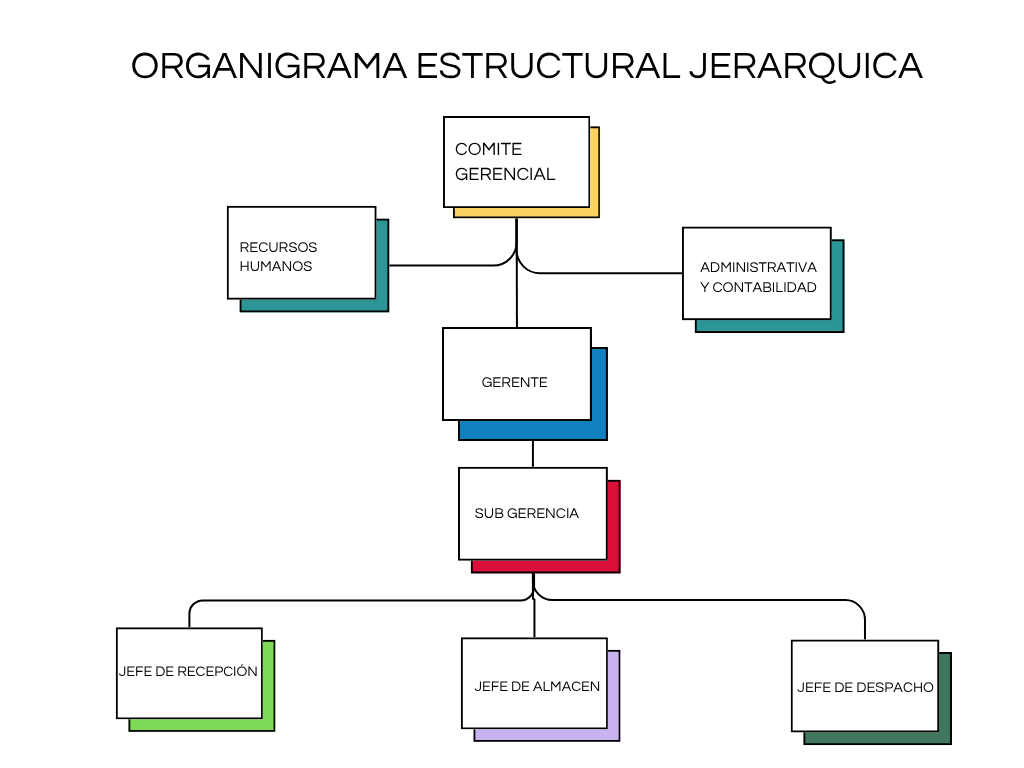
\includegraphics[width=5.5in,keepaspectratio]{media/image8.png}}
\end{center}

---

\section{Fase 3: Construcción y Pruebas del Proceso APO02}

\textbf{Objetivo:} Implementar los componentes diseñados del proceso APO02 y validar su funcionamiento antes de su despliegue formal.

\subsection{Desarrollo de Documentación Clave}
\textbf{Procedimientos Operativos Estándar (POEs)}
\textbf{Nombre:} POE para la Gestión de la Estrategia de TI (APO02)
\textbf{Contenido principal:}
* Frecuencia y agenda de sesiones estratégicas (trimestrales).
* Procedimiento para evaluar la alineación entre TI y Negocio.
* Métodos de priorización de iniciativas estratégicas.
* Criterios para revisar oportunidades tecnológicas.
* Uso obligatorio de BSC Designer para registrar, visualizar y evaluar KPIs estratégicos.
* Instrucciones para actualización del Plan Estratégico de TI.

\textbf{Guías de Usuario}
* \textbf{Guía 1:} Uso de BSC Designer para registrar y visualizar scorecards estratégicos.
* \textbf{Guía 2:} Flujo de trabajo del proceso APO02 (TO-BE), que detalla entradas, actividades, responsables, formatos y salidas.
* \textbf{Guía 3:} Revisión de KPIs y documentación de decisiones estratégicas.

\textbf{Materiales de Capacitación}
* \textbf{Presentación:} Introducción al nuevo proceso APO02.
* \textbf{Infografía del flujo TO-BE.}
* \textbf{Manual práctico:} Cómo realizar una revisión estratégica de TI.
* \textbf{Simulador de decisiones:} Mini casos para aplicar la matriz de alineación TI-negocio y priorizar acciones estratégicas.

\subsection{Configuración de Herramientas de Soporte}
\textbf{Plataforma: \href{https://bscdesigner.com}{BSC Designer}}
* \textbf{Scorecards configurados:} Mapa estratégico de TI cargado, KPIs por dominio (Financiero, Cliente, Proceso, Aprendizaje), línea base vs. metas estratégicas.
* \textbf{Dashboards personalizados:} Panel de control de metas de TI, reporte de alineación con negocio, y vista específica para el Comité Estratégico TI.
* \textbf{Usuarios configurados:} CIO, CTO, Comité, Gerentes de Producto, con accesos y permisos diferenciados para visualización y edición.

\subsection{Prueba Piloto del Proceso APO02}
\textbf{Alcance:} Ejecutar una iteración completa del proceso en un entorno controlado durante 1 mes.
\textbf{Actividades:}
1. Revisión estratégica simulada: el comité estratégico analiza los objetivos principales.
2. Evaluación de propuestas tecnológicas (ejemplo: integración del WMS con APIs de partners).
3. Uso de BSC Designer para registrar decisiones y actualizar KPIs.
4. Revisión final de la trazabilidad y validación.

\textbf{Resultados esperados de la prueba:}
* Validación de roles y responsabilidades (RACI en acción).
* Comprobación de la utilidad práctica del POE.
* Feedback de los usuarios sobre la usabilidad de BSC Designer.
* Identificación de mejoras menores antes del despliegue total en producción.

---

\section{Fase 4: Implementación y Transición del Proceso APO02}

\textbf{Objetivo:} Asegurar el despliegue efectivo del nuevo proceso de planificación estratégica de TI (APO02), su adopción por los usuarios clave y el monitoreo inicial para ajustes.

\subsection{Capacitación al Personal Involucrado}
\textbf{Población Objetivo:} CIO, CTO, Comité de Dirección de TI, Oficina de Proyectos (PMO), Líderes de Producto y Dueños de Proceso logístico, y Analistas de Planificación TI.
\textbf{Contenido de la Capacitación:}
* Objetivo y beneficios del nuevo proceso APO02.
* Flujo TO-BE y responsabilidades de la matriz RACI.
* Uso práctico de BSC Designer: carga, actualización y monitoreo de KPIs.
* Interpretación de scorecards y toma de decisiones basada en datos.

\textbf{Metodología:} Sesiones virtuales sincrónicas (Zoom o MS Teams), acceso a plataforma LMS con materiales de autoaprendizaje grabados, y simulaciones guiadas con ejercicios prácticos de carga de datos.
\textbf{Evidencia:} Registro formal de firmas y asistencia, evaluaciones de comprensión teórica, y reporte de certificación interna (``Usuarios capacitados APO02'').

\subsection{Despliegue del Proceso en Áreas Definidas}
\textbf{Ámbitos de despliegue inicial:} Comité Estratégico TI (nivel corporativo), Oficina de Proyectos PMO (planificación y seguimiento), y Líderes de plataformas tecnológicas clave (WMS, APIs).
\textbf{Actividades realizadas:}
* Activación oficial del calendario trimestral de planificación estratégica de TI.
* Implementación de plantillas estandarizadas de evaluación y priorización.
* Carga inicial de KPIs en scorecards activos (ej. exactitud de inventario, tiempo de picking, disponibilidad del sistema).

\textbf{Herramientas activas:} \textbf{BSC Designer} para scorecards operativos con metas SMART, y \textbf{Documentos compartidos} en la intranet para actas, POEs y matriz de iniciativas estratégicas.

\subsection{Gestión del Cambio y Adopción del Proceso}
\textbf{Plan de Gestión del Cambio:}
* \textbf{Mensaje Clave:} ``La estrategia TI en CO LOGISTIC S.A.C. ahora se mide y mejora con datos reales''.
* \textbf{Tácticas de comunicación:} Kick-off oficial presidido por el CIO, Newsletter mensual ``APO02 en acción'', y un repositorio centralizado con recursos didácticos y FAQs.

\textbf{Gestión de la resistencia:} Identificación de áreas con baja tasa de adopción de la herramienta, reforzamiento individualizado mediante mentoría 1:1 o coaching grupal, y reconocimiento público a los equipos operativos más alineados y comprometidos.

\textbf{Early Life Support y soporte técnico:} Soporte funcional directo en el uso diario de BSC Designer, canal de chat corporativo abierto para asistencia inmediata, y revisión quincenal del cumplimiento de actividades del flujo APO02.

---

\section{Fase 5: Operación y Medición del Proceso APO02}

\textbf{Objetivo:} Ejecutar de forma continua el proceso de planificación estratégica de TI (APO02), monitorear su rendimiento, y validar que se cumplen las metas y se mantiene o progresa hacia el \textbf{Nivel 5 de madurez}.

\subsection{Ejecución Continua del Proceso APO02}
\textbf{Actividades ejecutadas de forma cíclica:}

\vspace{0.3cm}
\setlength{\tabcolsep}{5pt}
\renewcommand{\arraystretch}{1.5}
\arrayrulecolor{TableLine}
{\def\LTcaptype{none}
\begin{longtable}[]{@{}
  >{\raggedright\arraybackslash}p{0.50\linewidth}
  >{\raggedright\arraybackslash}p{0.18\linewidth}
  >{\raggedright\arraybackslash}p{0.32\linewidth}@{}}
\rowcolor{DeepNavy}
\textcolor{white}{\textbf{Actividad Operativa}} & \textcolor{white}{\textbf{Frecuencia}} & \textcolor{white}{\textbf{Responsable Principal}} \\ \hline
\endhead
\rowcolor{LightGray}
Revisión de objetivos estratégicos de TI alineados al negocio. & Trimestral & CIO / Comité Estratégico TI \\ \hline
Análisis de entorno tecnológico y tendencias (PESTEL). & Semestral & Oficina de Estrategia \\ \hline
\rowcolor{LightGray}
Actualización y evaluación de scorecards en BSC Designer. & Mensual & Coordinador de Planeamiento TI \\ \hline
Sesiones de decisión estratégica y priorización de iniciativas. & Trimestral & Comité de TI \\ \hline
\rowcolor{LightGray}
Seguimiento de proyectos estratégicos alineados al plan. & Quincenal & Oficina de Proyectos (PMO) \\ \hline
\end{longtable}
}

\textbf{Documentos operativos activos en producción:} Plan Estratégico de TI actualizado, POE del proceso APO02, scorecards activos en BSC Designer, actas de sesiones mensuales de seguimiento, y el registro oficial de proyectos de TI priorizados.

\subsection{Recopilación y Análisis de Métricas}
Los indicadores estratégicos son recopilados de forma automatizada mediante la plataforma SaaS \textbf{BSC Designer}:

\textbf{KPIs Estratégicos APO02 (Activos):}

\vspace{0.3cm}
\setlength{\tabcolsep}{5pt}
\renewcommand{\arraystretch}{1.5}
\arrayrulecolor{TableLine}
{\def\LTcaptype{none}
\begin{longtable}[]{@{}
  >{\raggedright\arraybackslash}p{0.18\linewidth}
  >{\raggedright\arraybackslash}p{0.40\linewidth}
  >{\raggedright\arraybackslash}p{0.20\linewidth}
  >{\raggedright\arraybackslash}p{0.22\linewidth}@{}}
\rowcolor{DeepNavy}
\textcolor{white}{\textbf{Perspectiva}} & \textcolor{white}{\textbf{Indicador KPI}} & \textcolor{white}{\textbf{Meta SMART}} & \textcolor{white}{\textbf{Valor Actual (Ej.)}} \\ \hline
\endhead
\rowcolor{LightGray}
Financiera & ROI de proyectos TI (\%) & $\ge$ 15\% anual & 16.2\% \\ \hline
Cliente & Índice de satisfacción del cliente & $\ge$ 90\% semestral & 92.5\% \\ \hline
\rowcolor{LightGray}
Procesos Internos & \% de vulnerabilidades críticas activas & $\le$ 2\% mensual & 1.5\% \\ \hline
Procesos Internos & Tiempo promedio de picking y despacho & $\le$ 3 días & 2.6 días \\ \hline
\rowcolor{LightGray}
Talento & \% de personal técnico capacitado en WMS & 100\% anual & 95\% (en proceso) \\ \hline
Innovación & Nº de funcionalidades SaaS implementadas & $\ge$ 5 anuales & 3 (Q2) \\ \hline
\end{longtable}
}

\textbf{Métricas internas de control del proceso APO02:}

\vspace{0.3cm}
\setlength{\tabcolsep}{5pt}
\renewcommand{\arraystretch}{1.5}
\arrayrulecolor{TableLine}
{\def\LTcaptype{none}
\begin{longtable}[]{@{}
  >{\raggedright\arraybackslash}p{0.44\linewidth}
  >{\raggedright\arraybackslash}p{0.18\linewidth}
  >{\raggedright\arraybackslash}p{0.18\linewidth}
  >{\raggedright\arraybackslash}p{0.20\linewidth}@{}}
\rowcolor{DeepNavy}
\textcolor{white}{\textbf{Indicador de Proceso}} & \textcolor{white}{\textbf{Frecuencia}} & \textcolor{white}{\textbf{Valor Actual}} & \textcolor{white}{\textbf{Estado Operativo}} \\ \hline
\endhead
\rowcolor{LightGray}
\% de decisiones de inversión TI documentadas & Mensual & 98\% & Cumplido \\ \hline
\% de scorecards de TI revisados por periodo & Trimestral & 100\% & Cumplido \\ \hline
\rowcolor{LightGray}
\% de iniciativas tecnológicas alineadas al BSC & Trimestral & 88\% & En revisión \\ \hline
\end{longtable}
}

\textbf{Análisis de resultados:}
* Se observa un alto nivel de cumplimiento de los KPIs estratégicos en las áreas financieras y de procesos.
* Respecto al indicador de alineamiento estratégico de iniciativas (88\% frente a una meta de 95\%), se programó una sesión de revisión extraordinaria para adecuar los proyectos menores que operan fuera del alcance del BSC corporativo.

\subsection{Comparación con Metas y Nivel de Capacidad}
\textbf{Nivel de Capacidad Definido: Nivel 5 (Optimizado)}
* El proceso APO02 está formalmente estructurado, es medible, automatizado y se somete de forma permanente a ciclos de optimización y mejora continua.
* Los indicadores de performance se actualizan directamente desde fuentes en tiempo real y sirven como base científica para la toma de decisiones de inversión y de cambios estratégicos en TI.

\textbf{Evidencias de cumplimiento Nivel 5:}

\vspace{0.3cm}
\setlength{\tabcolsep}{6pt}
\renewcommand{\arraystretch}{1.5}
\arrayrulecolor{TableLine}
{\def\LTcaptype{none}
\begin{longtable}[]{@{}
  >{\raggedright\arraybackslash}p{0.45\linewidth}
  >{\raggedright\arraybackslash}p{0.55\linewidth}@{}}
\rowcolor{DeepNavy}
\textcolor{white}{\textbf{Requisito de Madurez Nivel 5}} & \textcolor{white}{\textbf{Evidencia Disponible}} \\ \hline
\endhead
\rowcolor{LightGray}
Uso consistente y automatizado de KPIs & Scorecards activos y dashboards integrados en la nube. \\ \hline
Toma de decisiones estratégica basada en datos & Actas de sesiones mensuales de análisis cuantitativo del comité. \\ \hline
\rowcolor{LightGray}
Optimización continua del proceso & Registro de lecciones aprendidas y control de cambios aplicados. \\ \hline
Alineamiento al Balanced Scorecard corporativo & Mapeo directo de objetivos tecnológicos y de negocio en el BSC. \\ \hline
\end{longtable}
}

---

\section{Fase 6: Optimización y Mejora Continua del Proceso APO02}

\subsection{Evaluación Periódica del Proceso}
\textbf{Frecuencia:} Trimestral (alineado con los ciclos de decisión del negocio).
\textbf{Métodos de evaluación:} Auditoría de cumplimiento interno de POEs, encuestas de usabilidad con administradores del BSC Designer, y entrevistas de control con miembros del Comité de TI.

\textbf{Resultados de la última evaluación:}

\vspace{0.3cm}
\setlength{\tabcolsep}{5pt}
\renewcommand{\arraystretch}{1.5}
\arrayrulecolor{TableLine}
{\def\LTcaptype{none}
\begin{longtable}[]{@{}
  >{\raggedright\arraybackslash}p{0.30\linewidth}
  >{\raggedright\arraybackslash}p{0.45\linewidth}
  >{\centering\arraybackslash}p{0.25\linewidth}@{}}
\rowcolor{DeepNavy}
\textcolor{white}{\textbf{Dimensión Evaluada}} & \textcolor{white}{\textbf{Indicador Cualitativo}} & \textcolor{white}{\textbf{Resultado Actual}} \\ \hline
\endhead
\rowcolor{LightGray}
Alineación Estratégica & \% de decisiones basadas en KPIs cuantitativos & 95\% \\ \hline
Medición Continua & Scorecards actualizados oportunamente por mes & 100\% \\ \hline
\rowcolor{LightGray}
Uso del POE & Cumplimiento estricto de actividades y flujos & 90\% \\ \hline
Satisfacción del Proceso & NPS de los usuarios funcionales de la plataforma & +75 (Excelente) \\ \hline
\end{longtable}
}

\subsection{Identificación de Oportunidades de Mejora}
* **Automatización Financiera:** Desarrollar APIs de integración directa para que BSC Designer recopile el cálculo de retorno financiero de proyectos enlazados al ERP contable.
* **Simplificación Visual:** Rediseñar la presentación gráfica de los dashboards estratégicos para sesiones ejecutivas rápidas.
* **Capacitación Estratégica:** Reforzar con capacitaciones en metodologías OKR y métricas avanzadas a mandos medios.

\subsection{Implementación de Mejoras}

\vspace{0.3cm}
\setlength{\tabcolsep}{5pt}
\renewcommand{\arraystretch}{1.5}
\arrayrulecolor{TableLine}
{\def\LTcaptype{none}
\begin{longtable}[]{@{}
  >{\raggedright\arraybackslash}p{0.28\linewidth}
  >{\raggedright\arraybackslash}p{0.38\linewidth}
  >{\raggedright\arraybackslash}p{0.34\linewidth}@{}}
\rowcolor{DeepNavy}
\textcolor{white}{\textbf{Mejora Propuesta}} & \textcolor{white}{\textbf{Objetivo del Cambio}} & \textcolor{white}{\textbf{Resultado Obtenido}} \\ \hline
\endhead
\rowcolor{LightGray}
\textbf{Mejora 1:} Integración de BSC Designer con Power BI. & Visualizar en tiempo real los KPIs financieros de almacén y despachos. & Reducción del tiempo manual de consolidación en un 40\%. \\ \hline
\textbf{Mejora 2:} Simplificación de plantillas de scorecard. & Facilitar la lectura de datos para miembros no técnicos del comité. & Aumento de la participación de la dirección y del consenso rápido. \\ \hline
\rowcolor{LightGray}
\textbf{Mejora 3:} Taller de toma de decisiones estratégicas. & Fortalecer capacidades del personal y adopción de la gobernanza de TI. & Satisfacción calificada con 4.8/5. Adopción del POE al 100\%. \\ \hline
\end{longtable}
}

\subsection{Alineación Continua con el SGTI}
* **Validación cruzada:** El Balanced Scorecard de TI y los objetivos comerciales de CO LOGISTIC S.A.C. se revisan de forma conjunta cada fin de trimestre, garantizando la consistencia estratégica.
* **Sostenibilidad:** El CIO y la Gerencia General ratificaron la continuidad del modelo trimestral de planificación bajo APO02 como estándar de gobierno institucional.

\end{document}
